\documentclass[manuscript]{aastex}

%% manuscript produces a one-column, double-spaced document:
%%\documentclass[manuscript]{aastex}

%% preprint2 produces a double-column, single-spaced document:
%% \documentclass[preprint2]{aastex}

%% \documentclass[preprint2,longabstract]{aastex}

% Final ApJ format
%\documentclass{emulateapj}

\usepackage{enumerate}
\usepackage{amsmath}
\usepackage{fourier}
\usepackage{framed}
\usepackage[usenames,dvipsnames]{color}
\usepackage{hyperref}

\definecolor{shadecolor}{named}{Goldenrod}
\definecolor{quotemark}{named}{Blue}
\newcommand{\asidebox}[1]{\begin{shaded}
{
\begin{picture}(0,0)(0,0)
      \put(-20,-3){\makebox(0,0){%
	  \scalebox{7}{\textcolor{quotemark}{\bfseries``}}}%
      }
    \end{picture}
   \textbf{Berian}: ``#1'' }
\end{shaded}
}


\newcommand{\ie}{\emph{i.e.}}
\newcommand{\vdag}{(v)^\dagger}
\newcommand{\myemail}{berian@berkeley.edu}
\newcommand{\N}{\mathcal{N}}
\newcommand{\bsmu}{\boldsymbol\mu}
\newcommand{\bsS}{\boldsymbol\Sigma}
\newcommand{\bsL}{\boldsymbol\Lambda}
\newcommand{\bsT}{\boldsymbol\Theta}



%% You can insert a short comment on the title page using the command below.
%\slugcomment{Notes for Josh Bloom \& Joey Richards}
\slugcomment{Draft dated \today}

\shorttitle{Bayesian Astrometry}
\shortauthors{James \& Bloom}


\begin{document}
\title{Bayesian Astrometry}
\author{J. B. James, J. S. Bloom, $\ldots$}
\affil{Astronomy Department, University of California, Berkeley CA, 94720-3411, USA}
%\affil{Dark Cosmology Centre, University of Copenhagen,\\ Juliane Maries Vej 30, 2100 Copenhagen \O, Denmark}
%\altaffiltext{1}{}

\begin{abstract}
We provide a scheme for probabilistic astrometry incorporating uncertainty distributions in matched object locations, as well in the astrometric mapping itself. We consider the case of astrometric calibration involving image alignment with linear transformations---translation, scaling and rotation---followed by non-parametric regression to account for localized distortions. The probabilistic mapping between frames that results can produce non-trivial distributions in the target frame, allowing for MCMC sampling to be used to propagate positions. Additionally, we present an accurate approximation to this process where the image alignment probability distribution can be described analytically, so that an astrometric query can be handled quickly and concisely, returning a location in the target frame that has its uncertainty specified in two spatial coordinates with covariance between them. We discuss generalizing this formalism to incorporate prior knowledge on astrometric components such as proper motion and parallax. An implementation of this scheme, including extensive documentation and examples, is available at \href{}{}%provide an explicit application to the case of bivariate normal distributions in the catalogue space of tie objects. %MCMC is used to generate a posterior estimate for the joint distribution of the transformation parameters. The use of distortion maps to represent the maximum likelihood transformation is also considered.
\asidebox{Text appearing in these boxes are guides for what to comment on.}
\end{abstract}

\keywords{}

\tableofcontents

\section{Introduction}

(JSB to contribute some opening text)

\subsection{Astrometry as a gaussian process}
In this work, we treat astrometry as a problem in vector field regression on the celestial sphere, where uncertainties may be present in the observational data and required in output. The regression has two parts: a transformation representing the alignment of frames that is applied uniformly across the image as an affine (parametric) mapping, and localized non-parametric distortions that are a residual to this background. This prescription leads us to model the astrometric mapping as a gaussian process: the map is an element in a space of functions characterized by a mean function---the background mapping---and a covariance representing the distortions to this mean. 

A short review of gaussian processes is provided within Section~\ref{sec:scheme}. Treating astrometry in this way carries a number of strong benefits: i) uncertainties can be derived that contain covariance between celestial coordinates; ii) all sources of error can be properly tracked, including the uncertain alignment between frames and the otherwise poorly understood distortion map; iii) regression from observed points to arbitrary locations within the field can incorporate variance throughout the image, extending even to highly non-trivial distortion effects; and iv) astrometry can be treated as Bayesian updating, allowing prior knowledge about proper motion and parallax (among other considerations) to be incorporated.

At its core, we require the process of astrometry to provide astronomers with positions transformed from one frame to another, with a concise summary of their uncertainties. While this process will in general yield non-trivial probability distributions that cannot be easily summarized, and being able to show such distributions visually is an important end, we also find that it is often possible to approximate the output simply and accurately as two-dimensional (i.e., bivariate) normal distributions in celestial coordinates, allowing for the inclusion of this technique in the data reduction process common to all members of the astronomical community.

\subsection{Previous work}
Summary of work within the astronomical community relevant to the goal of probabilistic astrometry (JSB? maybe goes at top of introduction?). Also, a summary of multi-response regression techniques, as we are extending these in interesting ways (JBJ, maybe just gets put in method section, as `previous work' subsections in the intro are uncommon in astronomy.)

\section{Scheme for probabilistic astrometry}\label{sec:scheme}
The astrometric mapping between a pair or sequence of astronomical data frames should be thought of an uncertain \emph{function}, and mappings between particular locations in each frame as evaluations of that function. This is because the mapping is only made apparent through the motions of matched objects between target frames, about which we might have some previous knowledge (for instance, in the form of parallax or proper motion), but all of which is inherently probabilistic. This article is concerned with how to handle the fundamental tasks of astrometry given this uncertainty.

We are able to make some statements about the nature of probabilistic astrometric mapping: firstly, that part of the transformation involves alignment of images, the result of the fairly simple linear operations of translation, rotation and scaling. Even this analytically tractable component will be inherently probabilistic when the locations of the objects used to define it are uncertain. The result is that an exact location in one frame may be uncertain and even highly non-trivial in another; a source with an uncertain location will compound this effect.

Secondly, imposed on top of this  parametric background are localized distortions produced by atmospheric or instrumental effects, whose physical origin is not, and likely cannot, be specified. Conventionally modeled with bivariate Chebyshev or Legendre polynomials, these distortions are in fact more flexibly treated in a non-parametric manner where the covariance between different positions within the image is specified explicitly. We are led to the choice of representing the astrometric mapping as a gaussian process, a probabilistic function defined by a mean function (the background mapping) and, by analogy with the multivariate normal treatment of data vectors, a covariance between pairs of spatial locations that controls the way a particular instance of the probabilistic function departs from the mean.

The space of mappings between frames is greatly constrained by observations in the form of matched objects in each frame. The problem of building a probabilistic astrometric mapping is then reduced to that of imposing these observations on any initial knowledge, and that of astrometric querying to the task of gaussian process regression. In the language of Bayesian probability, the prior knowledge of the mapping distribution is updated to a posterior distribution that incorporates the information provided by the data with their uncertainties. Then, querying is the result of propagating a point or spatial region in one frame through this function, mapping to a distribution in the target frame. 

This scheme provides an estimate of the posterior likelihood  for the astrometric solution between frames under the following assumptions: 
\begin{enumerate}[(i)]
\item two frames, $A$ and $B$, are used as comparators, where by convention $A$ is a reference frame, though this choice has no impact on the method;
\item objects within frames are characterized by bivariate normal distributions, with means $\boldsymbol\mu_i$ (the `location' of the object) and uncertainty ellipses defined by the covariance matrix $\boldsymbol\Sigma_i$;
\item the number of tie objects is known and all such pairs have been matched between the two frames, though the possibility of false matches is not excluded.
\end{enumerate}

Because astrometry is concerned with the motion (displacement) of objects between images, the uncertain function that is being estimated is a vector field, representing the transformation at each location of interest, with an associated covariance. If one wishes to know the location distribution of an object in the target frame, given its location (and distribution) in the initial frame, this is found by integrating over the vector field and associated covariance. %When necessary, we will refer to this paired field of vectors and covariances $\left\{\mathbf{v}(\mathbf{x}),\bsS(\mathbf{x})\right\}$ as a \emph{vector distribution field}.

Estimation of this field proceeds in the two parts outlined above: an affine background mapping component is estimated to account for global differences between the images that result from a relatively restricted set of linear transformations, specified by a seven-parameter model. The form of the likelihood distribution in this seven-parameter space can be left unspecified in general when sampling is used propagate between frames. From each sampling, the residual to the background transformation yields a local distortion field, which is characterized non-parametrically and with full covariance as a two-dimensional gaussian process whose mean is the background transformation. Chaining these two steps and tracking the sources of covariance that arise from them yields a likelihood distribution for the vector distribution field; this is the Bayesian astrometric solution.

Nothing in the formalism that follows requires assumptions about the probability distributions for the locations of observed matched pairs. However, it transpires that the assumption of bivariate normal object distributions makes the likelihood computation especially well behaved, so that many computations can be done without numerical integration. Moreover, this is the choice of distribution implicit when specifying a location with uncertainty in celestial coordinates, which is virtually the only representation of object positions used at the present time. This choice is adopted throughout this work. The remainder of this section gives an overview the parametric (\ref{ss:p}) and non-parametric (\ref{ss:np}) components of the scheme.
%Assumptions: bivariate distributions in catalogue space, restriction to transformations of translation, scaling and rotation, homogeneity of transformation across the frame.

\subsection{The parametric background}\label{ss:p}
In addition to the purely formal assumptions listed above, the following physical considerations are made:
\begin{enumerate}[(i)]
\item Image alignment consists of a global transformation that is homogeneous across the frame, i.e., the mapping is the same at every point;
\item the basis operations for the space of mappings between the two frames are: translation $\mathbf{x}\rightarrow \mathbf{x}' = \mathbf{x}+\Delta\mathbf{x}$, rotation about an arbitrary point $\mathbf{x}\rightarrow \mathbf{x}' = \mathbf{U}(\theta)\left(\mathbf{x}-\mathbf{x_0}\right)+\mathbf{x_0}$ and scaling  $\mathbf{x}\rightarrow \mathbf{x}' = \Lambda\mathbf{x}$, where scaling by negative values is allowed, corresponding to the image coordinates being flipped.
\end{enumerate}
This generates a seven-parameter model $\bsT_b = \left\{\Delta x, \Delta y, \theta, x_0, y_0, \Lambda_{xx},\Lambda_{yy}\right\}$, which transforms an initial point or probability distribution $p(\mathbf{x})$ to an aligned distribution $p_a(\mathbf{x};\bsT_b) \equiv T_{\bsT_b}\left[p(\mathbf{x})\right]$, where $T$ stands in for the form of the linear mapping transformation that will be made explicit in Section~\ref{s:background}; that section also treats the problem of likelihood estimation for this model in detail. Given matched catalogs of object locations with uncertainties, the parametric mapping can be expressed as a probability distribution $p\left(D; \bsT_b\right)$, the probability of the observed data $D$ for a specific choice of transformation parameters. For sampling, all that is required is the ability to compute the likelihood $\mathcal{L}(\bsT_b|D)$ for any choice of parameter set: an analytic form for the distribution as a whole is not needed.

When the input data have uncertainties associated with them, this background distribution will be spread out about its maximum value, giving rise to non-trivial target frame distributions even before local distortions are considered. For instance, consider the effect of an uncertain rotation parameter $\theta$. A fixed point (other than the centre of rotation) will be drawn out along an arc by this probabilistic mapping, an effect whose extent will increase the further the point is from the centre of rotation; similarly, uncertain scaling parameters will produce rectilinear distributions. By contrast, the effect on uncertain translation parameters is relatively benign, and in Section~\ref{sec:normapprox} we present ways this can be handled analytically in some settings.

But combining these uncertain transformations gives rise to target frame distributions that we should not aim to characterize explicitly. Likelihood sampling will allow us to define a contour in the target frame at some probability threshold that represents how a point or region is distributed. In particular, the exact expression
\begin{equation}
p_t(\mathbf{x}) = \int p_a(\mathbf{x};\bsT_b) dp(\bsT_b) = \int T_{\bsT_b}\left[p(\mathbf{x})\right]p(\bsT_b) d\bsT_b\label{eq:pt_background}
\end{equation}
for the posterior target frame probability distribution $p_t$ given a distribution $p$ in the initial frame and background mapping distribution $p_b$ can be sampled with the Metropolis-Hastings algorithm and characterized empirically to a desired level of precision.

\subsection{The non-parametric residual distortion map}\label{ss:np}
The parametric background is a first-order characterisation of the difference between image frames. The residuals to this background are local distortions that are manifestly non-parametric. We model this distortion map using a two-dimension gaussian process over the vector residuals at each location, training a covariance function to describe how a known mapping (\emph{i.e.}, from each of the tie objects) influences the estimation of the model in its neighborhood. 

A standard reference for gaussian processes is \citet{rasmussen2006gaussian}, whose development we follow here. A gaussian process may be thought of as a probability distribution $f(\mathbf{x})$ over the space of functions, characterized by a mean function $m(\mathbf{x}) = \mathbb{E}\left[f(\mathbf{x})\right]$ and a covariance function $k(\mathbf{x},\mathbf{x}') = \mathbb{E}\left[\left(f(\mathbf{x})-m(\mathbf{x})\right) \left(f(\mathbf{x}')-m(\mathbf{x}')\right)\right]$; we write
\begin{equation}
f \sim \mathcal{GP}(m(\mathbf{x}), k(\mathbf{x},\mathbf{x}')) = m(\mathbf{x}) + \mathcal{GP}(0, k(\mathbf{x},\mathbf{x}')).
\end{equation}
In probabilistic astrometry, the role of the mean function is played by the background image alignment transformation described in the previous subsection; local distortions are residuals to this mean. The generation of a distortion map proceeds by conditioning the function $k(\mathbf{x},\mathbf{x}')$ that describes the covariant relationship between pairs of spatial locations, using the observed residuals of the matched catalogs. This process of conditioning is described in Section~\ref{sec:gp}.

The description of a gaussian process as a probability distribution in the space of functions is abstract, and in practice what matters most is the values this function takes at specific locations: particularly, the locations of the observed matches on the one hand, and the locations within the image that we would like query astrometrically on the other. Using a gaussian process means that the values of the astrometric map at these sets of locations are jointly normally distributed, so that we can produce a conditional distribution for one set of locations (the ones we would like to regress) based on the others:
\begin{equation}
\left[\begin{array}{c} \mathbf{y} \\ \mathbf{y}_\ast\end{array}\right] \sim \left[\begin{array}{c} m(X) \\ m(X_\ast)\end{array}\right] + \mathcal{N}\left( \mathbf{0},
\left[\begin{array}{cc}
K(X,X) & K(X,X_\ast) \\
K(X_\ast,X) & K(X_\ast,X_\ast)
\end{array}\right] \right).
\end{equation}
The vector and matrix elements above are evaluations of the astrometric mapping at the observation ($X$) and target ($X_\ast$) locations. The vector of means is the background transformation mapping applied at the different sets of locations; the joint normal distribution on the right-hand side has mean zero and a covariance matrix who elements are themselves the matrices of the covariance function $k(\mathbf{x}, \mathbf{x}')$ evaluated at each pair of locations in the two sets $X$ and $X_\ast$, that is, 
\begin{equation}
K(X,Y) = \left[\begin{array}{cccc}
k(\mathbf{x}_1,\mathbf{y}_1)  & \cdots & k(\mathbf{x}_1,\mathbf{y}_m) \\
\vdots&\ddots&\vdots \\
k(\mathbf{x}_n,\mathbf{y}_1)&\cdots& k(\mathbf{x}_n,\mathbf{y}_m)
\end{array}\right];
\end{equation}
hereafter, we will write $K$ for $K(X,X)$, $K_\ast$ for $K(X_\ast,X)=K(X,X_\ast)^T$ and $K_{\ast\ast}$ for $K(X_\ast,X_\ast)$.

Because the values at all locations are jointly normally distributed, the astrometric mapping at the new locations $X_\ast$, given the observations of the mapping at locations in $X$, is itself normally distributed, with mean and covariance
\begin{equation}
 \overline{\mathbf{y}_\ast | \mathbf{y}} = m(X_\ast) + K_\ast K^{-1} \mathbf{y}; \quad C(\mathbf{y}_\ast | \mathbf{y}) = K_{\ast\ast} - K_\ast^T K^{-1} K_\ast.
\end{equation}

These expressions are the formulae for regressing the values of the astrometric map at query locations, given the observations in the matched catalogs. To reiterate, the mean displacement of the mapping is the background image alignment and the residuals are described completely by the covariance function $k(\mathbf{x},\mathbf{x}')$, about which we have said very little so far. The detailed consideration of this function will be postponed until Section~\ref{sec:gp}, but its basic properties are that it will be symmetric in inputs, stationary across the image frame and a function of the separation between input locations, so that it might instead be written $k(|\mathbf{x}-\mathbf{x}'|)$. Furthermore, we will presume that it is characterised by a limited set of parameters, called `hyperparameters' in this context, as they define a model within a space that is abstractly above the spatial plane of the image with which we are actually concerned. Training the covariance function with the observed data will produce a joint likelihood distribution on these parameters, in a manner analogous to the parameters of the background mapping model described in Section~\ref{ss:p}.

Ultimately, the hyperparameters $\bsT_\mathrm{HP}$ are joined to the background model parameters $\bsT_b$, yielding a higher-dimensional mapping space over which likelihood sampling takes place. This yields a probabilistic solution for the astrometric mapping between frames. Extending Equation~\eqref{eq:pt_background},
\begin{eqnarray}
 p_t(\mathbf{x}) & = & \int \int y_\ast\left[p(\mathbf{x}); \bsT_b, \bsT_\mathrm{HP}\right] p(\bsT_b) p(\bsT_\mathrm{HP}) d\bsT_p d\bsT_\mathrm{HP}  \\
 & = & \int \int \underbrace{T_{\bsT_b}\left[p(\mathbf{x})\right]}_\textrm{image alignment}+ \underbrace{\left(K_\ast K^{-1}\right)_{\bsT_\mathrm{HP}}\left(p(\mathbf{x}) - T_{\bsT_b}\left[p(\mathbf{x})\right]\right)}_\textrm{gaussian process residual distortion map} dp(\bsT_b) dp(\bsT_\mathrm{HP}).\label{eq:master}
 \end{eqnarray}

This is the master equation for the querying of an astrometric mapping defined by a matched pair of catalogs. The next two sections provide details on how the components of the probabilistic mapping are defined and how they can be sampled.

\subsection{Sampling from priors and posteriors}
Equation~\eqref{eq:master} describes an astrometric query as a process by which a possibly uncertain location in one frame is pushed to the target frame by a mapping that is itself uncertain. When little is known about the nature of the distributions for the locations or the mapping beyond a method to evaluate the likelihood for some choice of parameters, a likelihood sampling technique like the Metropolis-Hastings algorithm can be used to generate samples in the target frame.

%It is conceivable that in some circumstances additional parameters should be added to incorporate proper motion, parallax or further known instrument distortions, though these are not considered at present. 

\section{Image alignment: MCMC likelihood estimation}\label{s:background}
The previous section described the process through which a probability distribution in the initial frame is propagated into the target frame with a probabilistic mapping that is defined by matched pairs of objects with associated uncertainties. This section describes the first component of this mapping, the linear transformation of image alignment that acts globally across the frame. Except where noted, it is assumed that objects in the matched catalogs have their locations specified by bivariate normal distributions, as this is the only case relevant to astronomers at the present time and makes the presentation substantially more concrete. Nothing within the formalism explicitly requires this assumption, however; for non-gaussian distributions on the observed object locations, the process of likelihood sampling is simply extended to incorporate those distributions as well.

\subsection{Linear transformation of bivariate normal distributions}
A bivariate normal distribution is an excellent representation of an uncertain celestial position at the current level of precision available to astronomers. Writing $\mathcal{N}(\bsmu, \bsS)$, the probability density function for the object's location is
\begin{equation}
p(\mathbf{x}) = \frac{1}{2\pi |\bsS|^{1/2}} e^{-\frac{1}{2}(\mathbf{x}-\bsmu)^T \bsS^{-1} (\mathbf{x}-\bsmu)}.
\end{equation}
In the context of an image frame, $\mathbf{x}$ might be a vector of the pixel coordinates; or it could represent the right ascension and declination of the object. We assume that all objects in the matched catalogs have location distributions of this form and label the two frames under comparison $A$ and $B$.

\begin{figure}[htbp]
\centering
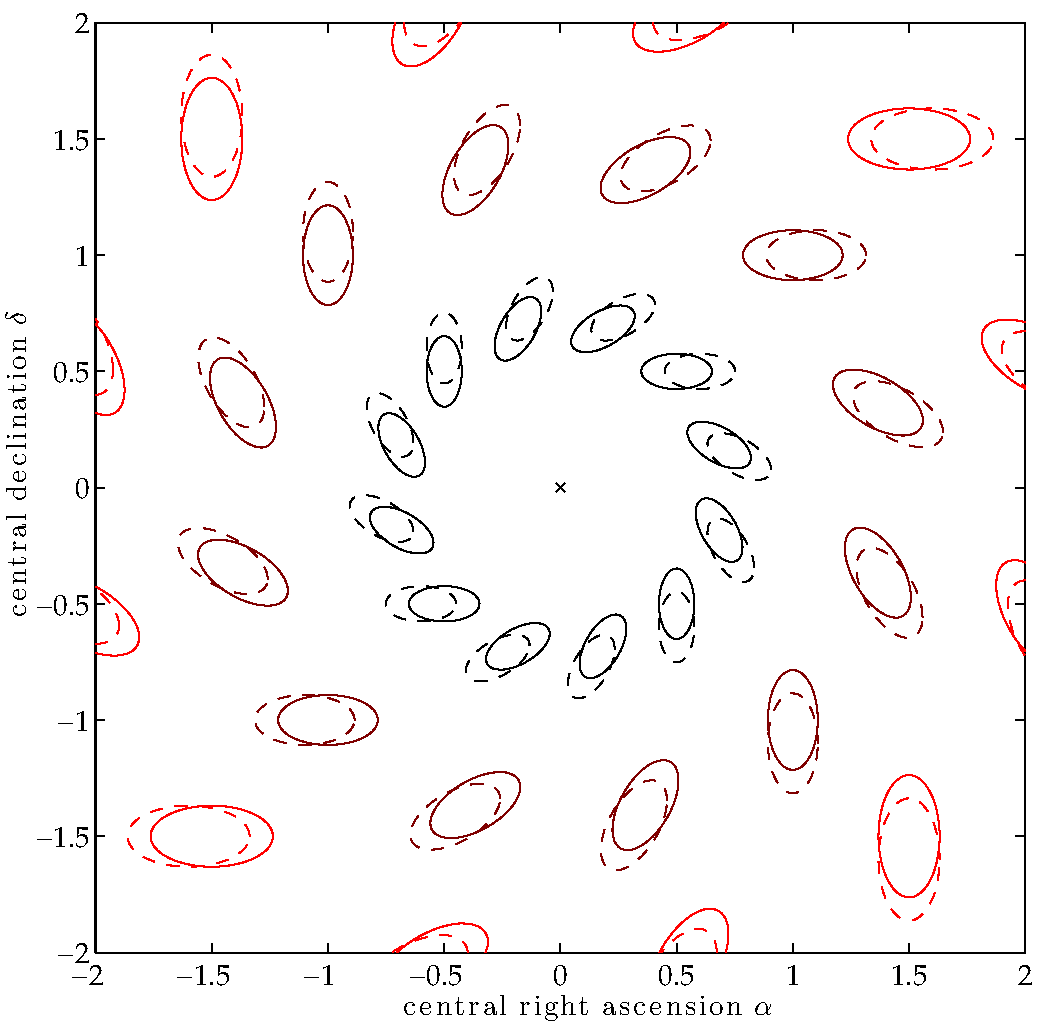
\includegraphics[width=\linewidth]{figures/gaussian_mappings.pdf}
\caption[Mappings of a bivariate gaussian under the three basis operations considered in this work: translation (dashed), scaling (color) and rotation.]{Mappings of a bivariate gaussian under the three basis operations considered in this work: translation (dashed), scaling (color) and rotation. In each case the template bivariate $\mathcal{N}\left(\left[
\begin{smallmatrix}
1 \\ 1
\end{smallmatrix}
\right],\left[ 
\begin{smallmatrix}
0.1 & 0 \\ 0 & .05
\end{smallmatrix}
\right]
\right)$ is transformed according to the prescription of equation (\ref{eq:bivar_map}).}\label{fig:gaussian_mappings}
\end{figure}
Let $p_A^i\sim\N(\bsmu_A,\bsS_A)$ represent the likelihood distribution in frame $A$ for the $i$th matched object and similarly for $p_B^i$. It is straightforward to generate the corresponding frame $B$ distribution under the seven-parameter transformation $\bsT_b = \left\{\Delta\bsmu, \theta, \mathbf{x}_0, \bsL\right\}$ using the spectral decomposition of $\bsS=\mathbf{V}\mathbf{D}\mathbf{V}^{-1}$:
\begin{eqnarray}
 p^i_{\tilde{B}}(\mathbf{x}) \equiv T_{\bsT_b}\left[p^i_{B}(\mathbf{x})\right]& = & \Delta\bsmu + \bsL^{1/2}\mathbf{U}(p^i_B-\mathbf{x}_0) + \mathbf{x}_0 \\ & \sim & \N\left( U(\bsL\bsmu+\Delta\bsmu-\mathbf{x}_0)+\mathbf{x}_0,(\mathbf{U}\mathbf{V})(\bsL^{1/2}\mathbf{D})(\mathbf{U}\mathbf{V})^{-1}\right). \label{eq:bivar_map}
 \end{eqnarray}
Here, $\mathbf{V}$ is the matrix of eigenvectors of $\bsS$ and $\mathbf{D}$ the diagonal matrix of corresponding eigenvalues; the transformation composes scaling, translation and rotation (in that order) and operates on the mean of the gaussian in the way it would on a single point, while the error ellipse is transformed by rotating the principal axes of the error ellipse with the rotation matrix $U$ of angle $\theta$ and scaling each of the principal axis sizes, which are given by the eigenvalues. Figure~\ref{fig:gaussian_mappings} shows the transformations of a template bivariate gaussian generated by the basis translation, rotation and scaling mappings where the center of rotation $\mathbf{x}_0$ has been placed at the centre of the frame.

\subsection{Likelihood construction}
This section describes how to evaluate the relative likelihood value for a mapping $\bsT_b$ given the object distributions in the two frames. The $B$ frame distributions are transformed in the manner described above, so that it remains to decide how the correspondence between tie objects in the reference and mapped frames is evaluated.

Given a tie object reference distribution $p^i_A$ and a trial mapped distribution $p^i_{\tilde{B}}$, the likelihood contribution from the tie pair is given by a measure of separation between the two distributions. The natural choice of distance function for the two distributions in this context is the Bhattacharaya distance,
\begin{equation}
 D_B = -\log\left( \int_\mathcal{A}\sqrt{p q}d\mathbf{x}\right),
 \end{equation}
i.e., the integral over the frame of the geometric mean distribution. This definition provides $D_B=0$ when $p = q$ and the integral is interpreted geometrically as a measure of overlap between the two distributions. In the limit where the object's location is known exactly in one frame, the distance gives a normalised measure of the deviation of that value from the centre of the comparison distribution. \footnote{An alternative is the Kullback-Leibler divergence \[D_{KL}(p|q) = \int_{-\infty}^{\infty} p(x) \log\frac{p(x)}{q(x)} dx \] that is popular in feature separation. In a Bayesian context it should be interpreted as an evaluation of the information gain in going from the prior to the posterior, which is distinct to what we aim for in astrometry. This, together with it being asymmetric in $p$ and $q$, leads us to prefer the Bhattacharaya distance; in a practical setting the difference is unimportant. Note, though, that neither of these quantities defines a metric in the formal sense.}
For a pair of bivariate gaussians distributions, the distance $D_B$ permits analytic expression:
\begin{equation}
D_B(p^i_A,p^i_{\tilde{B}}) = \frac{1}{8}(\bsmu_A-\bsmu_{\tilde{B}})^T\bsS^{-1}(\bsmu_A-\bsmu_{\tilde{B}}) + \frac{1}{2}\log\left(\frac{|\bsS|}{\sqrt{|\bsS_A||\bsS_{\tilde{B}}|}}\right),\quad\textrm{where }\bsS = \frac{\bsS_A+\bsS_{\tilde{B}}}{2},
\end{equation}
so that for a background mapping $\bsT_b$, the likelihood computation given the data is
\begin{equation} \mathcal{L}(\bsT_b|D) \propto \exp\left(-\sum_i D_B\left(p^i_A,p^i_{\tilde{B}(\bsT_b)}\right)\middle/2\right).\label{eq:background_likelihood}
\end{equation}

\section{Residual distortion map: a gaussian process approach}\label{sec:gp}
The work in the previous section addresses the first part of the problem, providing a global mapping between image frames. The task is now to characterize probabilistically the resulting residual distortion map in a manner that can be smoothly joined to the task of estimating the background, so that both parts---parametric and non-parametric---can be carried out in unison. 

We argue for treating the residual distortion map as a two-dimensional gaussian process over the vector components at each location, which requires the specification of a covariance function and outputs a mean vector (the mean astrometric solution) and covariance for the vector components. This section describes this covariance function in detail, particularly with regard to gaussian process regression of a vector, which has been the subject of only limited study within the machine learning literature. 

\subsection{Vector-output gaussian processes}
Much of the relevant literature on gaussian processes deals with the regression of a scalar-valued function. In these cases, the role of the covariance function is to describe how the different spatial locations (termed `inputs') are correlated so that the values of the regression function at those locations (termed `outputs') can be relayed to new locations. A particular choice of covariance function, written
\begin{equation}
k(\mathbf{x},\mathbf{x}') = \sigma_l^2 e^{(\mathbf{x}-\mathbf{x}')^2/2l^2} \equiv \sigma_l^2 \tilde{k}(\mathbf{x},\mathbf{x}')
\end{equation}
and termed the `square exponential' covariance function, is commonly encountered and is the general form that we pursue here; the unweighted covariance function $\tilde{k}$ will be needed when we consider vector output.  The two hyperparameters $l$ and $\sigma_l$ control the scale and amplitude of the correlations between locations, respectively. Using all pairs of points within the sets $X$ and $X_\ast$ of the input and regression locations, the matrices populated with scalar values $K$, $K_\ast$ and $K_{\ast\ast}$ can be constructed from evaluations of the covariance function.

When the outputs are not scalar-valued but vector-valued, a consideration of a different kind arises. Now, in addition to the correlation between different spatial locations, the correlation between the components of the outputs must also be evaluated; in the case of astrometry, there are two components for the two spatial directions. We handle this by splitting the role of the scale and amplitude hyperparameters: within the image frame, the scale parameter is isotropic and so remains a scalar $l$, but the amplitude should be generalized to a symmetric $2\times2$ matrix, so that the covariance function is matrix valued:
\begin{equation}
\left[\begin{array}{cc}
k_{xx}(\mathbf{x},\mathbf{x}') & k_{xy}(\mathbf{x},\mathbf{x}') \\ 
k_{yx}(\mathbf{x},\mathbf{x}') & k_{yy}(\mathbf{x},\mathbf{x}')
\end{array} \right] = 
\left[\begin{array}{cc}
\sigma_{l,xx}^2 & \sigma_{l,xy} \\
\sigma_{l,yx} & \sigma_{l,yy}^2
\end{array} \right]  e^{(\mathbf{x}-\mathbf{x}')^2/2l^2} \equiv \bsS_ke^{(\mathbf{x}-\mathbf{x}')^2/2l^2} ,
\end{equation}
subject to the constraints $\sigma_{l,xy}=\sigma_{l,yx}$ and, unless a clear reason for discriminating between spatial directions is apparent, $\sigma_{l,xx}=\sigma_{l,yy}$.

This matrix represents the correlation between each pair of components at just one particular pair of locations $\mathbf{x}$ and $\mathbf{x}'$. Generalizing the construction of the covariance function matrices $K$, $K_\ast$ and $K_{\ast\ast}$:
\begin{eqnarray}
\mathbb{K} = \tilde{K} \otimes \bsS_k & = & \left[\begin{array}{cccc}
\tilde{k}(\mathbf{x}_1,\mathbf{y}_1)  & \cdots & \tilde{k}(\mathbf{x}_1,\mathbf{y}_m) \\
\vdots&\ddots&\vdots \\
\tilde{k}(\mathbf{x}_n,\mathbf{y}_1)&\cdots& \tilde{k}(\mathbf{x}_n,\mathbf{y}_m)
\end{array}\right] \otimes \left[\begin{array}{cc}
\sigma_{l,xx}^2 & \sigma_{l,xy} \\
\sigma_{l,yx} & \sigma_{l,yy}^2
\end{array} \right] \\
& = & 
\left[\begin{array}{ccc}
\tilde{k}(\mathbf{x}_1,\mathbf{y}_1)\bsS_k &\cdots & \tilde{k}(\mathbf{x}_1,\mathbf{y}_n)\bsS_k \\
\vdots & \ddots &\vdots \\
\tilde{k}(\mathbf{x}_n,\mathbf{y}_1)\bsS_k &\cdots & \tilde{k}(\mathbf{x}_n,\mathbf{y}_n)\bsS_k \\
\end{array}\right];
\end{eqnarray}
here, $\otimes$ is the Kronecker matrix product, so that each element of $\mathbb{K}$ is the $2\times2$ matrix of covariance between spatial components weighted by the unnormalised scalar covariance function value. While the nested matrices appear conceptually, in implementation $\mathbb{K}$ is simply a $2n\times2n$ matrix, for $n$ input locations.\footnote{This formulation is most similar to one suggested by~\citet{bonilla-et-al-nips-07}, who note that when the observed data are known precisely the gaussian process regression decouples into two independent processes---one on each of the vector components---a property known as autokrigeability in the field of geostatistics.} Likewise, if regression is occurring to $m$ new locations, $\mathbb{K}_\ast$ and $\mathbb{K}_{\ast\ast}$ will be $2n\times2m$ and $2m\times2m$ respectively.

The gaussian process regression equations are straightforwardly generalized
\begin{equation}
 \overline{\mathbf{y}_\ast | \mathbf{y}} = m(X_\ast) + \mathbb{K}_\ast \mathbb{K}^{-1} \mathbf{y}; \quad \mathbb{C}(\mathbf{y}_\ast | \mathbf{y}) = \mathbb{K}_{\ast\ast} - \mathbb{K}_\ast^T \mathbb{K}^{-1} \mathbb{K}_\ast,
\end{equation}
where
\begin{equation}
\mathbf{y} = \left[ (y_{1,x},y_{1,y}), (y_{2,x},y_{2,y}),\ldots,(y_{n,x},y_{n,y}) \right]^T
\end{equation}
is reshaping of the $n\times2$ observed output spatial components at the $n$ observed input locations. Similarly, the regression yields a vector of length $2m$ ordered as pairs of spatial components at each of the $m$ regression locations, with all correlations between and vector components and locations accounted for. Finally, each element of $\mathbb{C}$ is a $2\times2$ covariance matrix, and the diagonal of $\mathbb{C}$ is a sequence of $m$ $2\times2$ covariance matrices describing the uncertainty in the regressed vector mapping at each output location.



\subsection{Measurement uncertainties on matched catalogue data}
When measurement uncertainties are present in the observations, this information must be propagated through the estimation of the astrometric mapping. For a pair of matched object locations $(p_A^i, p_B^i)$ that are both bivariate normal distributions, the mapping vector they define is also bivariate normal, with mean $\bsmu_A^i - \bsmu_B^i$ with uncertainty $\Sigma_A^i+\Sigma_B^i$. For a particular background mapping parameter choice $\bsT_b$, the residual to the background mapping---which is $\mathbf{y}_i$ in the gaussian process---will remain bivariate normal, with mean vector $(\bsmu_A^i - \bsmu_B^i) - T_{\bsT_b}\left[\bsmu_A^i\right]$ and covariance $T_{\bsT_b}\left[\Sigma_A^i+\Sigma_B^i\right]$.

This transformed covariance matrix $\Sigma_r^i$, representing the uncertainty in the vector residual to the background mapping, can be incorporated into the gaussian process regression using a formulation that is standard for scalar-output gaussian processes:
\begin{equation}
 \overline{\mathbf{y}_\ast | \mathbf{y}} = m(X_\ast) + \mathbb{K}_\ast (\mathbb{K}+\Sigma_r\mathbb{I})^{-1} \mathbf{y}; \quad \mathbb{C}(\mathbf{y}_\ast | \mathbf{y}) = \mathbb{K}_{\ast\ast} - \mathbb{K}_\ast^T (\mathbb{K}+\Sigma_r\mathbb{I})^{-1} \mathbb{K}_\ast,
\end{equation}
where $\Sigma_r\mathbb{I}$ represents a diagonal matrix whose $n$ diagonal elements are the residual mapping uncertainties $\Sigma_r^i$ for each of the $n$ pairs of matched object locations. Both the regressed vector field and the estimate of its uncertainty will now incorporate the uncertainty in the initial observations.

\subsection{Covariance hyperparameters}
In the vector-output gaussian process described above, there are three hyperparameters: $l$, the isotropic scale of the covariance function; $\sigma^2_{l}\equiv \sigma^2_{xx}=\sigma^2_{yy}$, the amplitude of gaussian process regression; and the new parameter $\sigma_{xy}$ describing the amplitude of the correlation between the vector output components. Though gaussian process regression may be thought of as non-parametric in the space of the image, it is in fact hyperparametric and these three parameters can be conditioned in just the same way as the parameters to the background mapping. The log-likelihood for a choice of hyperparameters $\bsT_\mathrm{HP}$ is
\begin{equation}
-2\log\mathcal{L}(\bsT_\mathrm{HP}|D) = \mathbf{y}^T(\mathbb{K}+\Sigma_r\mathbb{I})^{-1} \mathbf{y} + \log|\mathbb{K}+\Sigma_r\mathbb{I}| + \log2\pi,
\end{equation}
which can be used both to define a maximum-likelihood choice of hyperparameters and in likelihood sampling to generate samples of points from the distribution in the target frame.

This completes the description of the necessary formalism for Bayesian astrometric sampling. As presented, an input set of matched catalogues whose data are object locations expressed as bivariate normal distributions will define a total likelihood expression $\mathcal{L}(\bsT_b|D) + \mathcal{L}(\bsT_\mathrm{HP}|D)$. Sampling this likelihood, perhaps with the additional step of sampling the location in the initial frame when it is specified as a distribution, will produce a sequence of locations in the target frame that can be treated as an estimate of the posterior astrometric mapping solution.

\section{Normal approximation to astrometric mapping}\label{sec:normapprox}
Likelihood sampling is the most comprehensive method of generating an astrometric mapping in the target frame, but frequently an approximation the distribution in the target frame will be desired so that the astrometric query can return a concise result. This can be achieved with the addition of two assumptions, neither of which is burdensome:
\begin{enumerate}[(i)]
\item When the uncertainties on the observational data are small relative to the scale of the image, the background mapping probability distribution will be well approximated by a seven-dimensional multivariate normal distribution in the parameters $\bsT_b$;
\item furthermore, when the background mapping distribution is well constrained about a maximum likelihood value $\bsT_b^\mathrm{ML}$, the gaussian process hyperparameters can be conditioned just once, setting $p(\bsT_\mathrm{HP})$ to a delta function at $\bsT_\mathrm{HP}^\mathrm{ML}$.
\end{enumerate}

If these requirements are satisfied, then the master astrometric regression equation~\eqref{eq:master} is analytically tractable. With the observational data and their uncertainties expressed as probabilistic vectors between matched objects locations, with mean vectors $\mathbf{y}_i$ and stacked covariances $\bsS_r^i$, then from an initial frame distribution $p(\mathbf{x})\sim\mathcal{N}(\bsmu,\bsS)$, the output distribution in the target frame $p_t(\mathbf{x})$ will be well approximated by a bivariate normal distribution with mean mapping 
\begin{equation}
\bsmu_t = T_{\bsT_b^\mathrm{ML}}\left[\bsmu\right]+\left(\mathbb{K}_\ast (\mathbb{K}+\bsS_r\mathbb{I})^{-1}\right)_{\bsT_\mathrm{HP}^\mathrm{ML}}\left(\mathbf{y} - T_{\bsT_b^\mathrm{ML}}\left[\mathbf{y}\right]\right),\label{eq:approx_mu}
\end{equation}
and covariance
\begin{equation}
\bsS_t = \left[\mathbb{K}_{\ast\ast} - \mathbb{K}_\ast^T (\mathbb{K}+\bsS_r\mathbb{I})^{-1} \mathbb{K}_\ast\right]_{\bsT_\mathrm{HP}^\mathrm{ML}} + \bsS_b + \bsS,\label{eq:approx_sigma}
\end{equation}
where the terms in this expression correspond (from left-to-right) to the covariance contributions of the gaussian process, the uncertain background mapping and the initial frame uncertainty.

\subsection{Image alignment probability distribution}
All of the terms in the expressions~\eqref{eq:approx_mu} and~\eqref{eq:approx_sigma} are defined by either the observational data ($\mathbf{y}$, $\bsS_r$), the location of the query ($\bsmu$, $\bsS$) or the parameter distributions $p(\bsT_b)\sim\mathcal{N}(\bsT_b^\mathrm{ML},\bsS_{\bsT_b})$ and $p(\bsT_\mathrm{HP})\sim\delta(\bsT_\mathrm{HP}^\mathrm{ML})$. Proceeding with the assumption that the distribution for the background mapping parameters will be multivariate normal, we must decide how to extract an estimate of the covariance contribution within the image plane $\bsS_b$ from the covariance matrix of the larger parameter space $\bsS_{\bsT_b}$.

The covariance matrix for the background mapping parameters, $\bsS_{\bsT_b}$ can be estimated using the likelihood expression~\eqref{eq:background_likelihood}, by sampling the likelihood values along each parameter axis in the vicinity of the maximum. In particular, the elements of the precision matrix $L = \left[-\bsS_{\bsT_b}\right]^{-1}$are given by
\begin{eqnarray}
L''_{ij} \equiv \frac{d^2L}{d\theta_id\theta_j}= &&\left.\left[\mathcal{L}\left(\bsT_b^\mathrm{ML}+\epsilon\hat{e}_i+\epsilon\hat{e}_j\right) - \mathcal{L}\left(\bsT_b^\mathrm{ML}+\epsilon\hat{e}_i-\epsilon\hat{e}_j\right) - \right.\right.\\ && \left.\left.\mathcal{L}\left(\bsT_b^\mathrm{ML}-\epsilon\hat{e}_i+\epsilon\hat{e}_j\right) + \mathcal{L}\left(\bsT_b^\mathrm{ML}-\epsilon\hat{e}_i-\epsilon\hat{e}_j\right)\right]\middle/4\epsilon^2\right.,
\end{eqnarray}
where $\hat{e}_k$ is the unit parameter vector for a step along the $k$th dimension and $\epsilon$ is a small number. This procedure of numerical differentiation returns a precision matrix whose inverse fully characterizes the normal approximation to the background mapping distribution~\citep{gelman2004bayesian}.

Even when the background mapping distribution is represented in this manner, the propagation of this uncertainty into the target frame cannot be derived analytically. A special case is when the uncertainty in the translation parameters is the primary source of uncertainty, in which case the conditional covariance matrix constructed for these two parameters (i.e., given the maximum likelihood values for the others) will be a good approximation to $\bsS_b$.

More commonly, the covariance contribution from the background mapping should be estimated by sampling the multivariate normal $p(\bsT_b)$ some number of times and estimating the covariance in the target frame of the resulting point set.

%Even in this case, however, finding the maximum likelihood or maximum a posteriori transformation is useful. In addition to the maximum likelihood background mapping, the likelihood distribution in the neighborhood of the maximum is characterized. 

%\subsection{Maximum likelihood solution for the parametric background}

\subsection{Covariance stacking}

\section{Applications}
How can the construction of these distributions be painlessly used to improve the quality of science that is carried out?

\subsection{Mock data}
\begin{figure}[h]
\centering
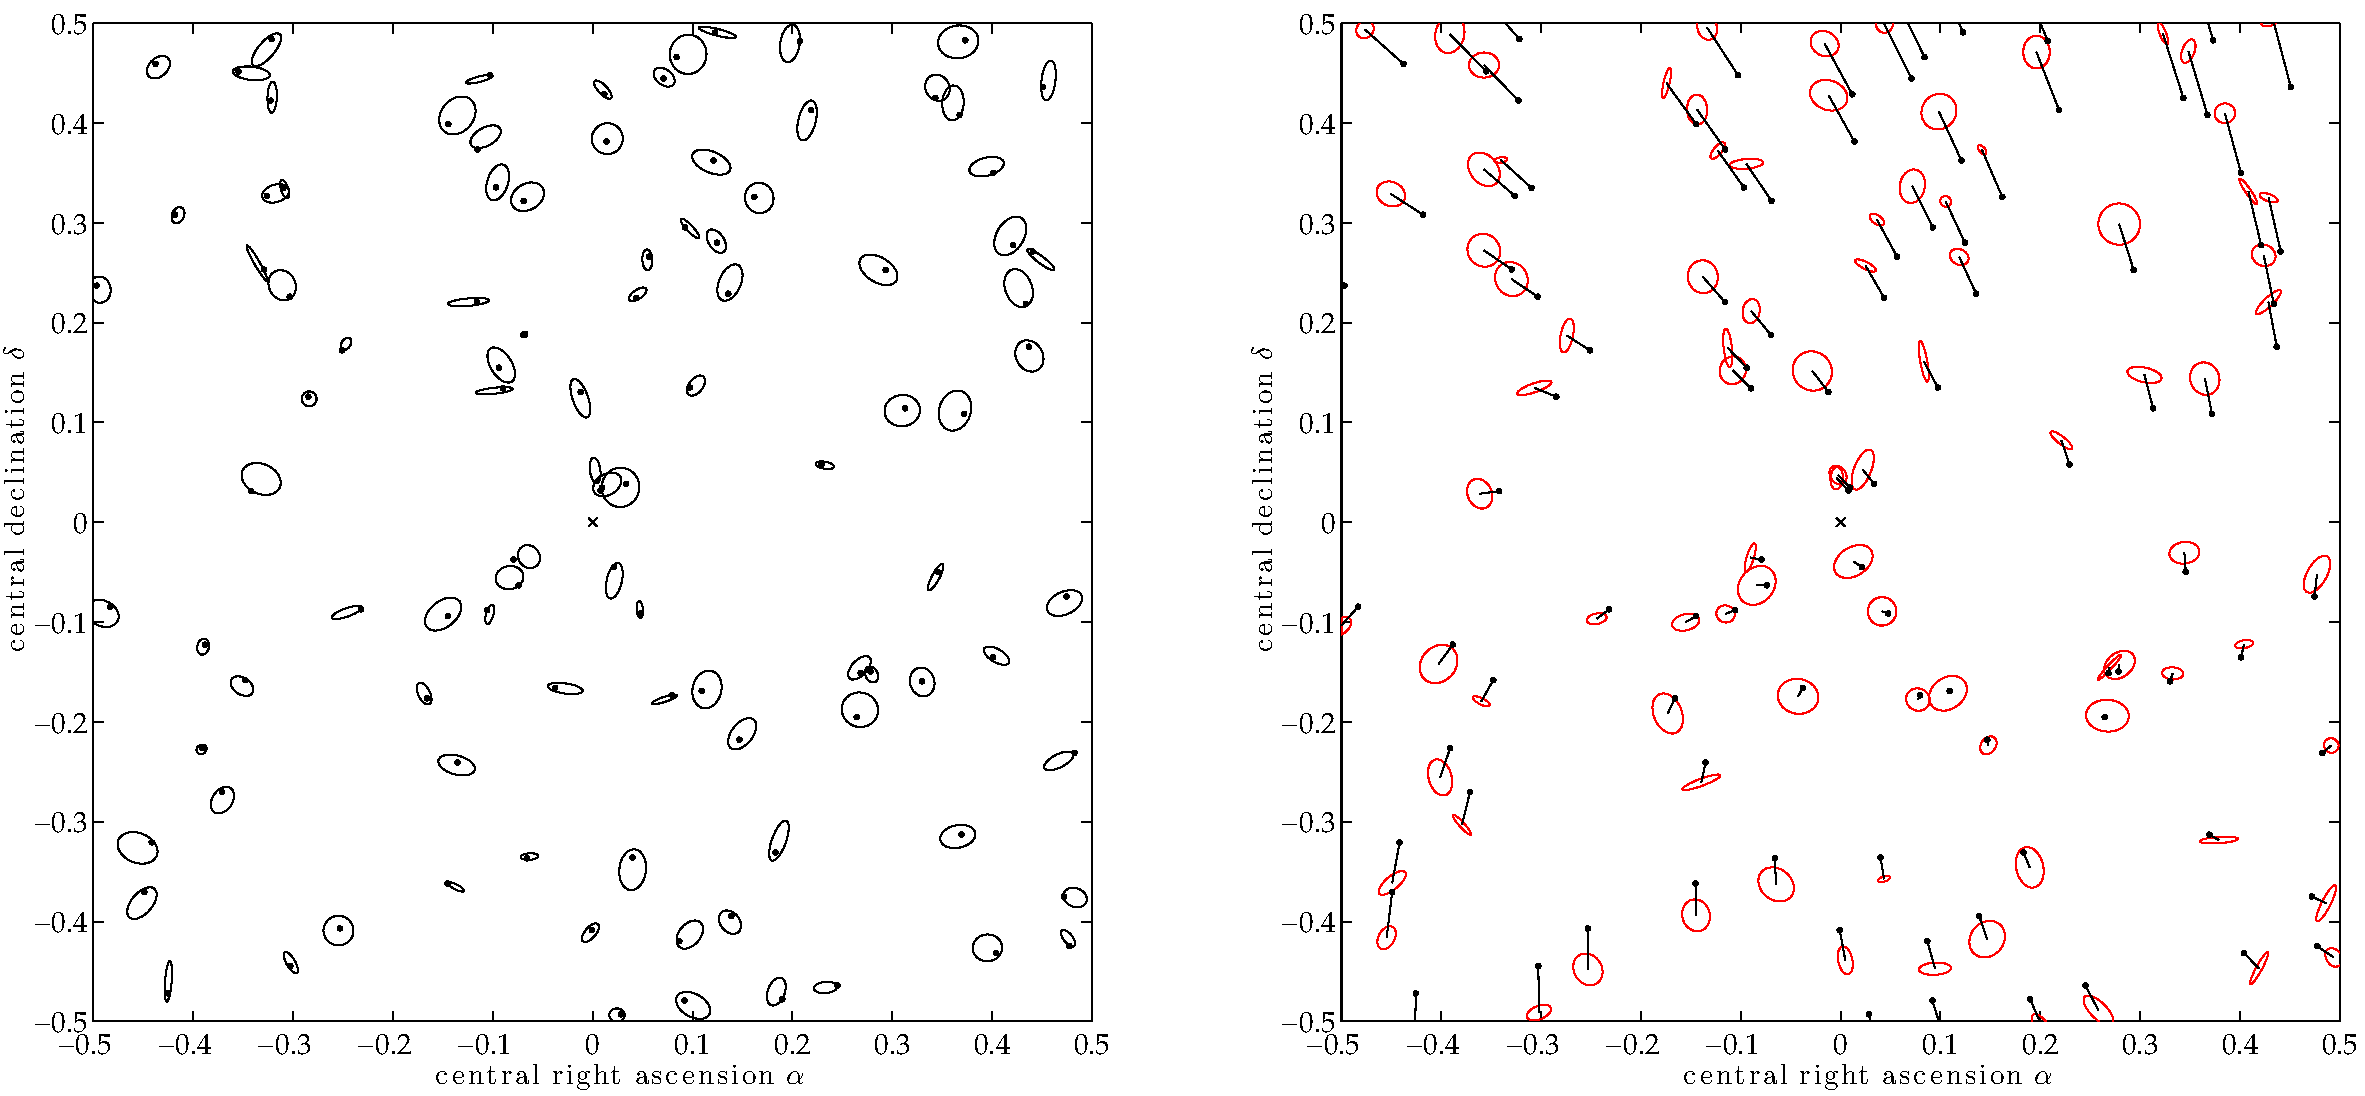
\includegraphics[width=\linewidth]{figures/test_data.pdf}
\caption{The mock data used in the application of the Bayesian astrometry scheme. \emph{Left:} A set of 100 bivariate gaussians (ellipses) are placed within the image frame and sampled (points) to generate the starting locations for the mapping. \emph{Right:} The starting locations (points) are transformed according to equation (\ref{eq:bivar_map}) and used as the central positions for objects in the new image frame, which are then assigned random bivariate gaussian covariance matrices (ellipses). }\label{fig:test_data}
\end{figure}
A pair of mock frames consisting of $n=100$ tie objects is generated in the following manner
\begin{enumerate}[(i)]
\item the set of object locations in frame $A$ are drawn using $\bsmu^i_A\sim U\left([-\frac{1}{2},\frac{1}{2}]\times[-\frac{1}{2},\frac{1}{2}]\right)$;
\item each location is assigned bivariate gaussian uncertainty distribution $\mathcal{N}\left(\bsmu^i_A,\bsS^i_A\right)$, where the covariance matrix $\bsS^i_A$ is determined from the widths $\left(\sigma_x^i,\sigma_y^i\right)\sim U[0.001,0.1]$ and rotated by angle $\theta^i_A\sim U[0,2\pi)$;
\item a random point is drawn from each bivariate gaussian distribution to provide the starting location $\bsmu^i_B$ for the mapping into frame $B$, as shown in the left panel of Figure~\ref{fig:test_data};
\item in the new image frame, these points are subject to the same random transformation, giving $\bsmu^i_{\tilde{B}}\sim\mathbf{U}(\bsL\bsmu + \Delta\bsmu)$, where $\mathbf{U}$ is the matrix of rotation by angle $\theta\sim U(0,\pi/50]$ about the origin, the scaling parameters are $\left(\Lambda_{xx}, \Lambda_{yy}\right)\sim U[0.9,1,1]$ and the translation is $\Delta\bsmu\sim U\left([-0.02,0.02]\times[-0.02,0.02]\right)$;
\item the transformed object locations are assigned bivariate gaussian uncertainty distributions $\mathcal{N}\left(\bsmu^i_{\tilde{B}},\bsS^i_{\tilde{B}}\right)$ following the same prescription as before.
\end{enumerate}
The two mock images with object locations and uncertainty distributions are shown in Figure~\ref{fig:test_data}.

\begin{figure}[h]
\centering
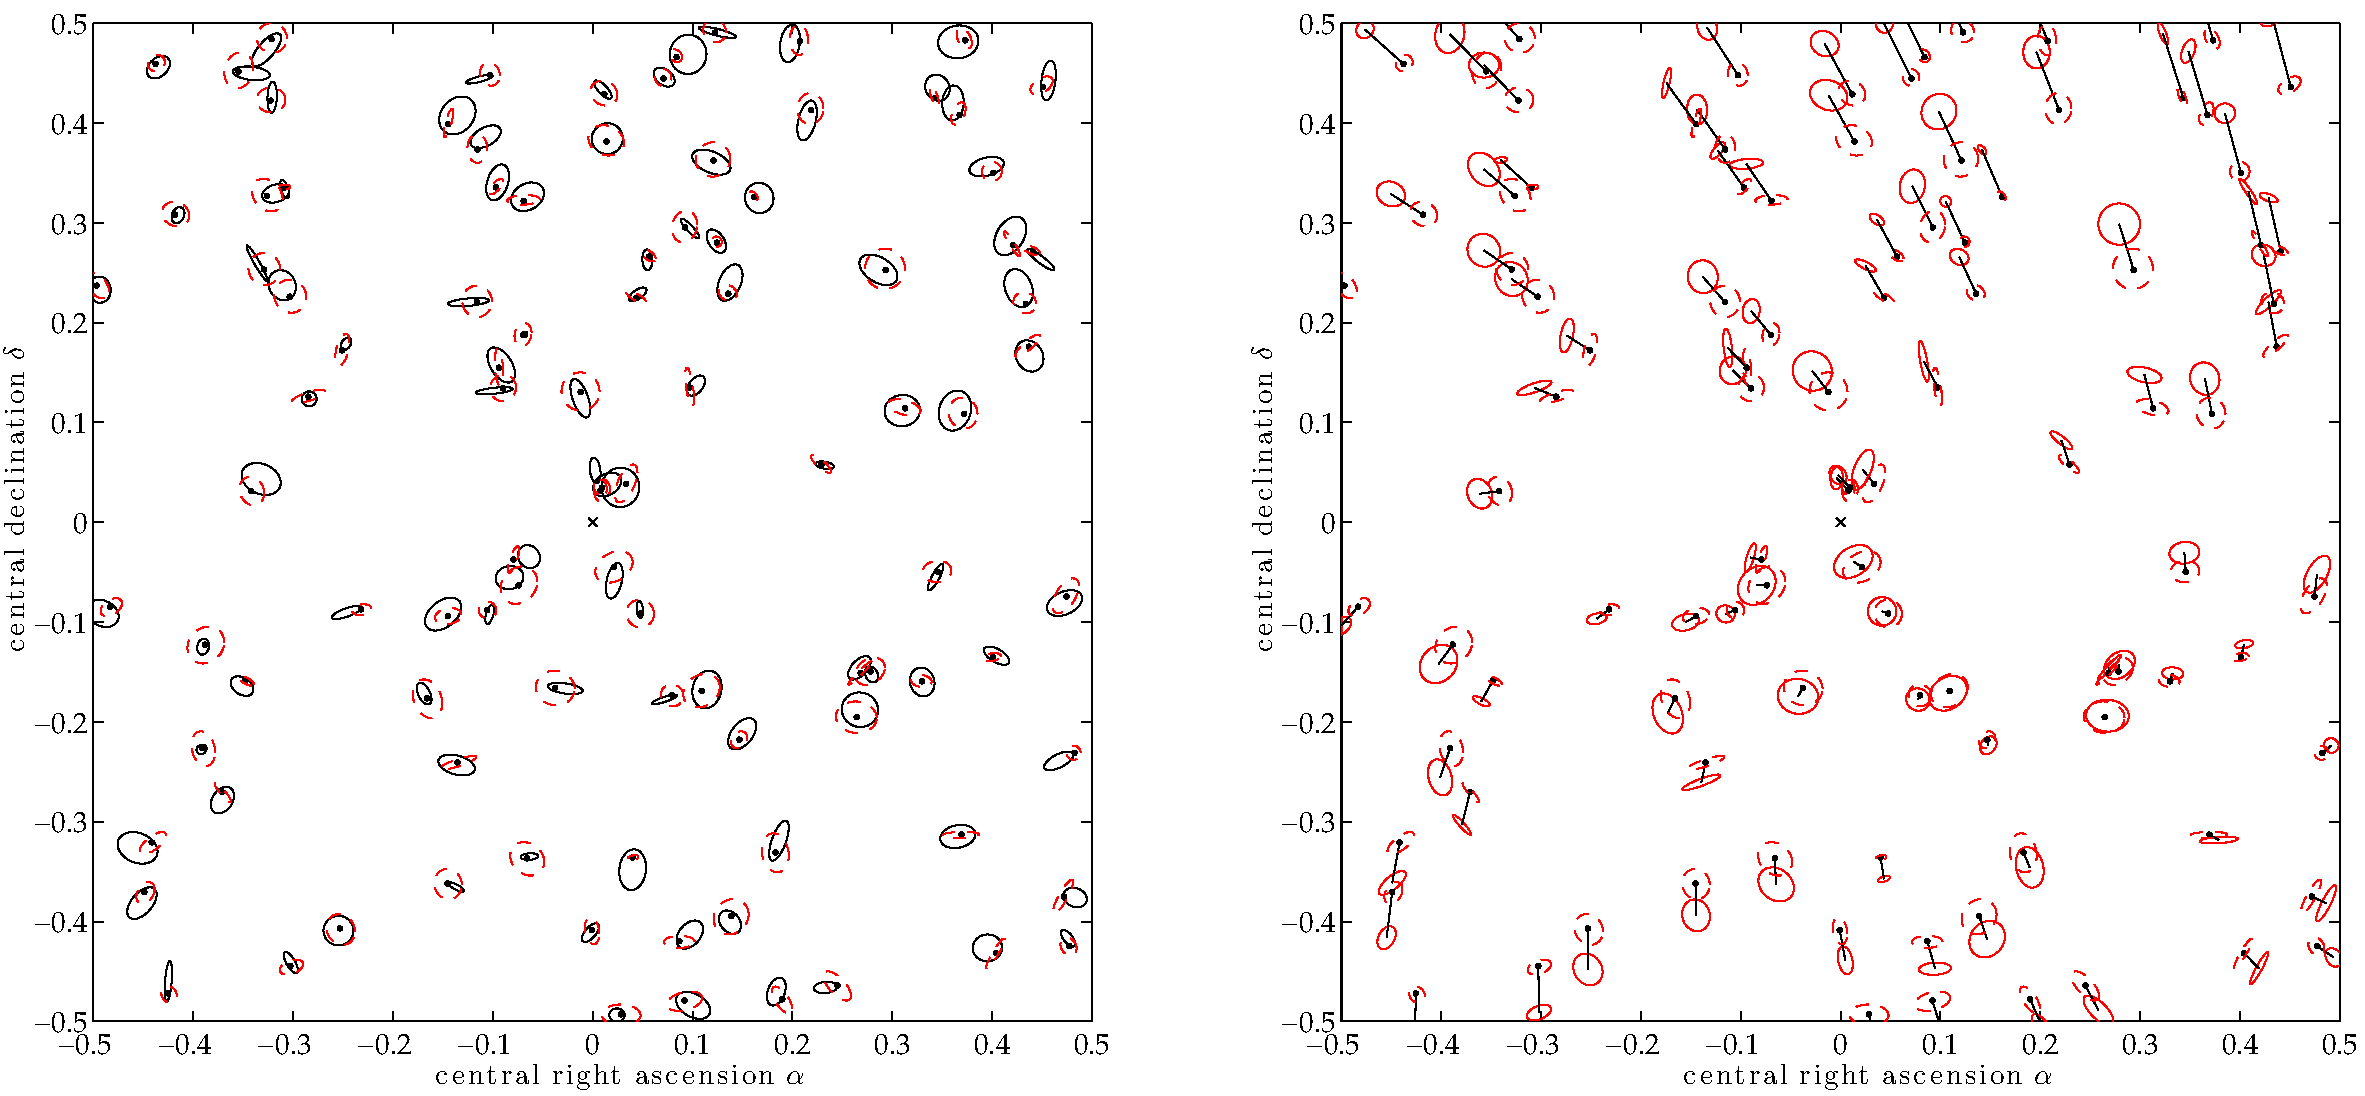
\includegraphics[width=\linewidth]{figures/test_solution.pdf}
\caption{The maximum likelihood (ML) solution for the mapping between frames given the mock test data. \emph{Left:} The $A$ frame object distributions (black) with the ML map of the $B$ frame tie object distributions superimposed. \emph{Right:} The starting locations (points) are transformed according to equation (\ref{eq:bivar_map}) and used as the central positions for objects in the new image frame, which are then assigned random bivariate gaussian covariance matrices (ellipses). }\label{fig:test_solution}
\end{figure}
Before considering the production of the the full likelihood distribution for the parameter set $\bsT_b$, the `best' mapping is examined in the form of the maximum likelihood value of $\mathcal{L}(\bsT_b)$. This peak is found by minimizing  $-2\log\mathcal{L}$, starting from the identity map $(\mathbf{0},0,\mathbf{1})$, a  computation that is $\mathcal{O}(n)$ in the number of tie objects.
\footnote{As is usual for Nelder-Mead optimization, the resulting extremum is somewhat sensitive to the choice of starting point. The best-fitting translation seems quite robust, but the maximum likelihood scaling and rotation do vary a little. This is irrelevant in the MCMC prescription.}

%\subsection{MCMC prescription}
\begin{figure}[h]
\centering
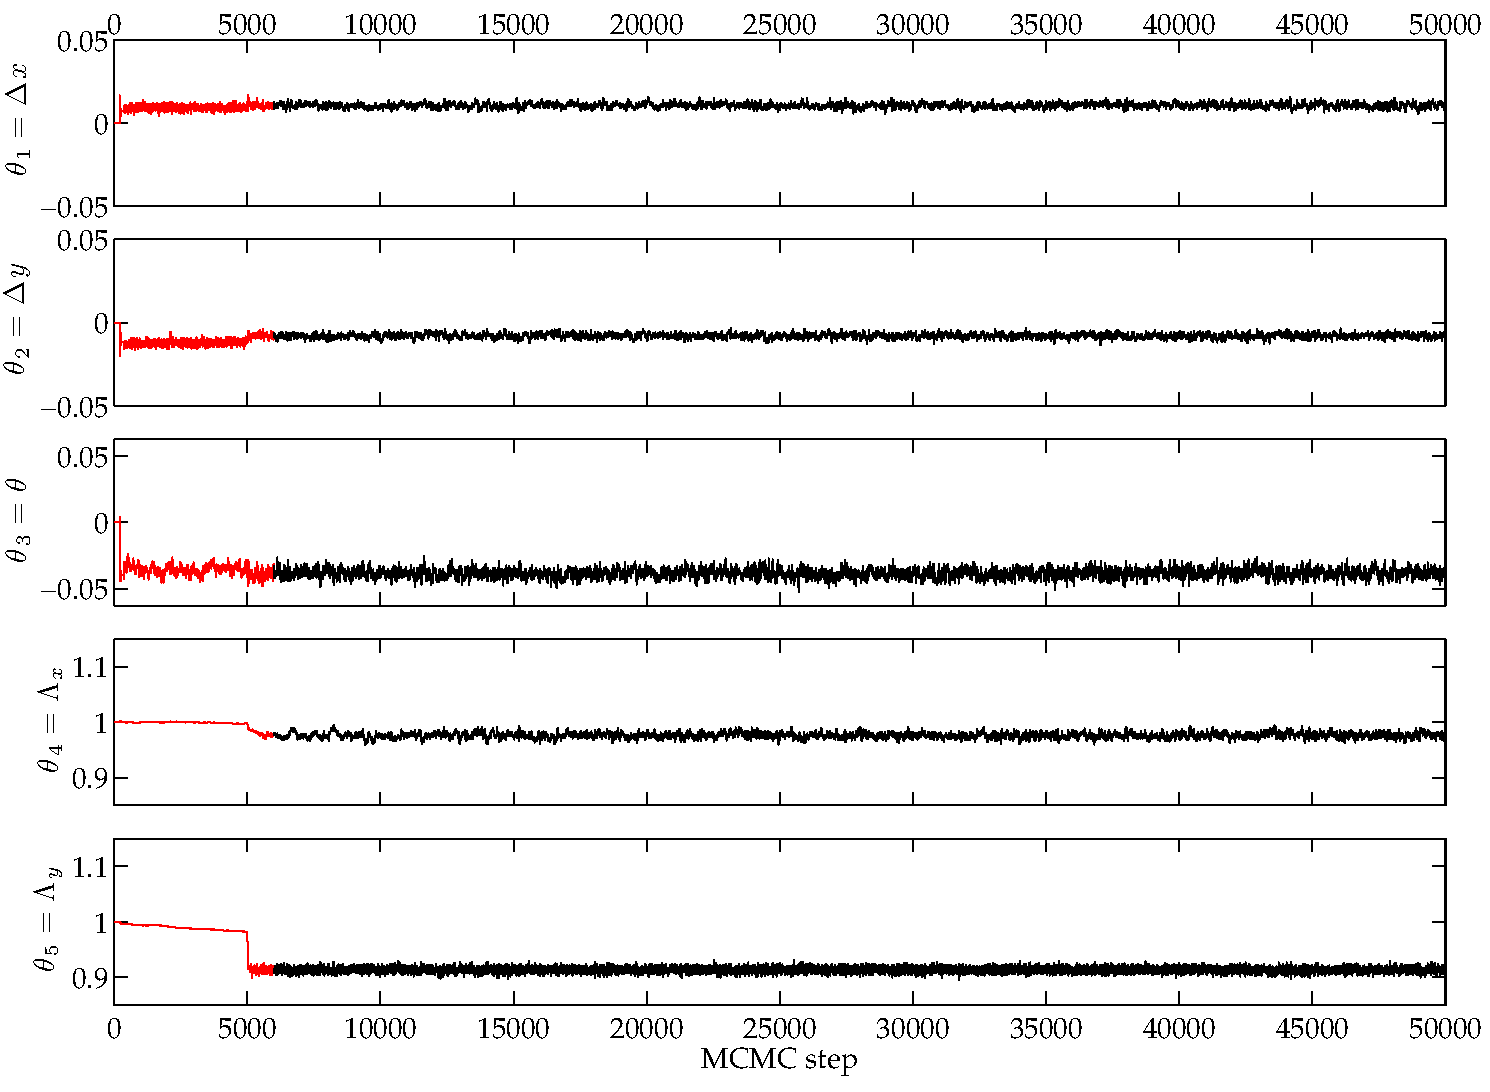
\includegraphics[width=\linewidth]{figures/chain_test.pdf}
\caption{Chains for the translation $(\Delta x, \Delta y)$, rotation $\theta$ and scaling $(\Lambda_x,\Lambda_y)$ parameters, with the burn-in period indicated with red colouring. The range of the parameter value axis has been narrowed from the width of the uniformed prior so that variability within the chain is visible.}\label{fig:chains}
\end{figure}
This section described how this work incorporates the full MCMC estimate of the likelihood distribution. A chain on 50,000 steps was run on the mock data with loglikelihood function $D_B$, with a burn-in period of 6,000 steps. The prior distributions for each of the five parameters $(\Delta x, \Delta y, \theta, \Lambda_x, \Lambda_y)$ are uniform with limits set equal to the limits on the input uniform random distributions in steps (ii) and (iv) of the mock data production scheme. 

\footnote{H. Haario, M. Laine, A. Mira and E. Saksman (2006), \emph{DRAM: Efficient adaptive MCMC}, Statistics and Computing \textbf{16}, pp. 339-354; P. J. Green and A. Mira (2001b), \emph{Delayed rejection in reversible jump Metropolis-Hastings}, Biometrika, Vol. 88, pp. 1035-1053; H. Haario, E. Saksman and J. Tamminen (2001), \emph{An adaptive Metropolis algorithm}, Bernoulli \textbf{7}, pp. 223-242}. Figure~\ref{fig:chains} shows the progress of each parameter throughout the chain.

\subsubsection{Maximum likelihood solution}
The barycentric mean of the joint parameter sets over the length of the chain  provides an estimate of the maximum likelihood solution:
\[ \hat\bsmu = \left[\widehat{\Delta x}, \widehat{\Delta y},\hat\theta, \widehat{\Lambda_x},\widehat{\Lambda_y}\right] = \left[0.0105,  -0.0080,  -0.0383,    0.9761,    0.9136\right]; \]
\[\hat{\boldsymbol\sigma}\times 10^2 = \left[0.1414,    0.1384,    0.3425,    0.4924,    0.4396\right] \]
for reference, this mapping is satisfyingly close to the (inverse of) the random mapping used to transform the $A$ frame object locations (prior to their being assigned $B$ frame uncertainty distributions), which is
\[ \left[-{\Delta x}, -{\Delta y},-\theta, 1/{\Lambda_x},1/{\Lambda_y}\right] = \left[ 0.0102,   -0.0086,   -0.0391,    0.9782,    0.9116\right].\]

The task now is to convert the chain into a generalized mapping distribution that convert object locations or distributions in one image frame to distributions in the other. The approach taken here is to assume that the five-dimensional likelihood distribution of the mapping parameters is multivariate normal, so that the marginalized parameter distributions and pairwise covariance between parameters will determine the likelihood distribution in full. 

\paragraph{Covariance matrix of likelihood distribution}
\begin{figure}[h]
\centering
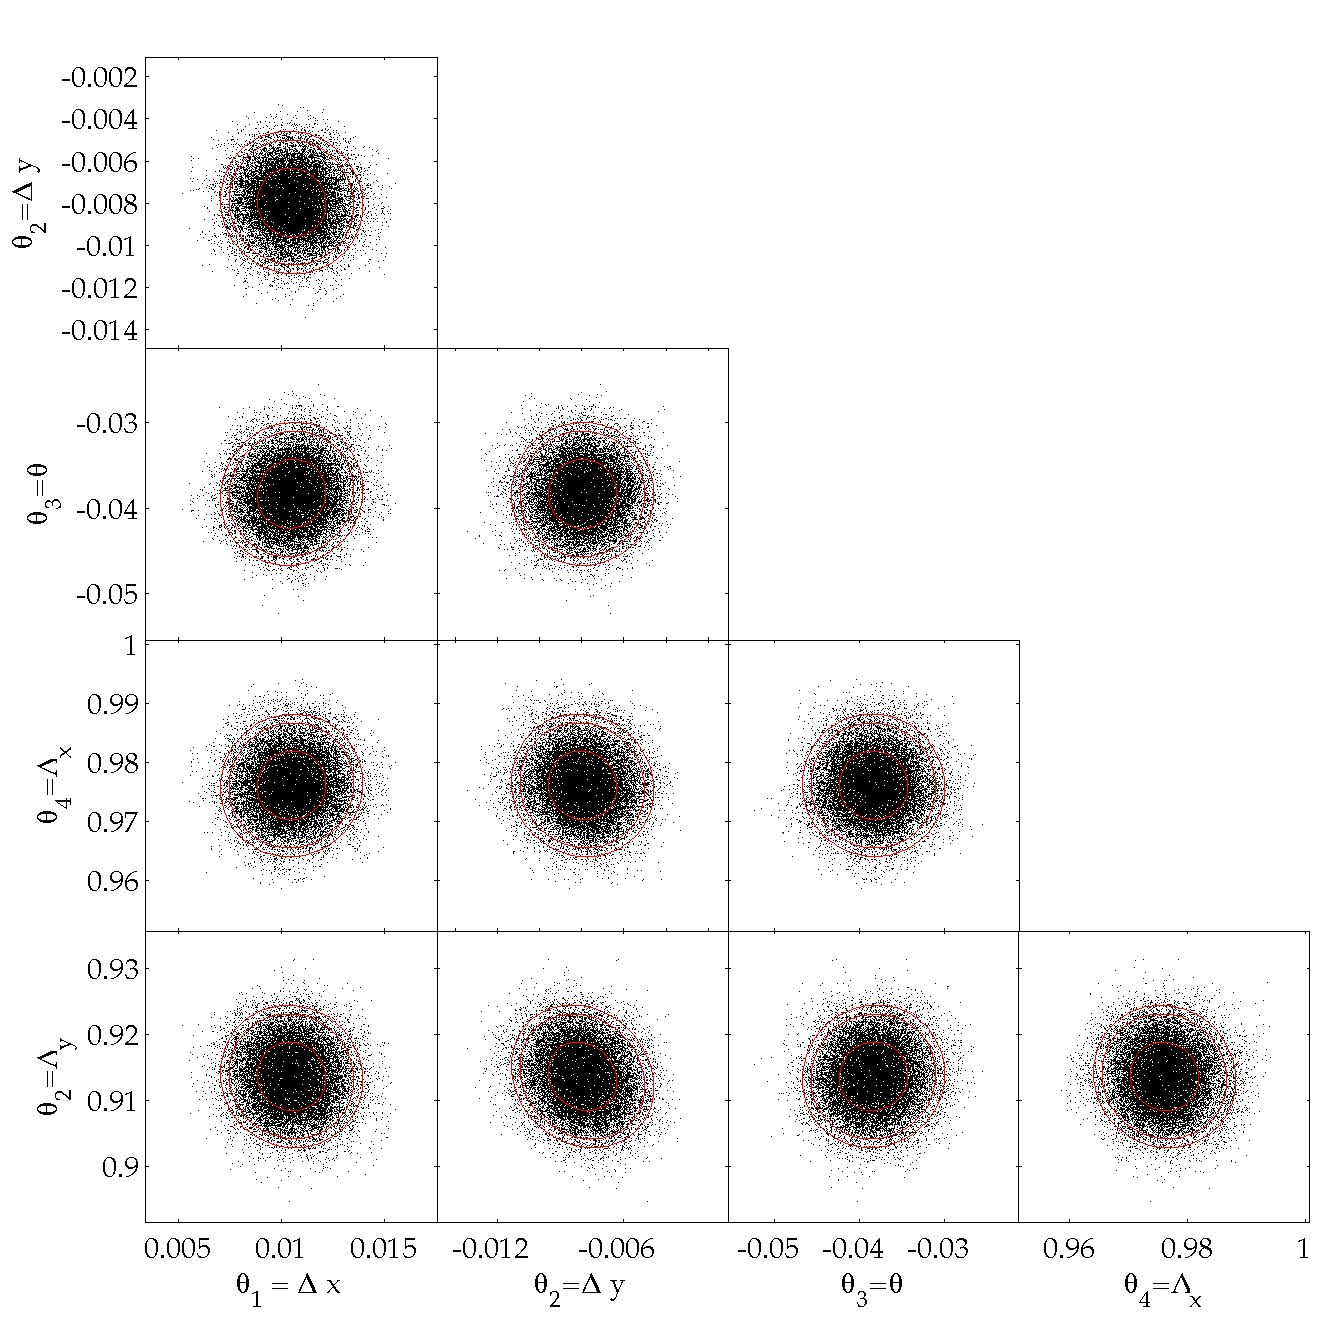
\includegraphics[width=\linewidth]{figures/jointL.pdf}
\caption{Pairwise joint likelihood distributions for transformation parameters, with each point representing a step in the chain and ellipses containing 50\%, 90\% and 95\% of the distribution.}\label{fig:jointL}
\end{figure}
The joint likelihood distributions of each pair of mapping parameters is shown in Figure~\ref{fig:jointL}. Under the assumption that the mapping likelihood distribution is multivariate normal, the covariance matrix elements $\bsS_{ij}$ are equal to the covariance $\sigma_{ij}$ between all pairs of parameters. This covariance matrix is:
\[ C(i,j)\times10^6 = \left(\begin{array}{ccccc}
2.0065&-0.075375&0.29147&0.22954&-0.28978\\
-0.075375&1.924&-0.0012628&-0.40617&-0.9144\\
0.29147&-0.0012628&11.7927&-0.31664&0.65299\\
0.22954&-0.40617&-0.31664&24.0556&-1.1182\\
-0.28978&-0.9144&0.65299&-1.1182&19.3468\\
\end{array}\right)\]

It is apparent that the parameters are mostly uncorrelated:
\[\frac{C(i,j)}{\sqrt{C(i,i)C(i,j)}} = \left(\begin{array}{ccccc}
1&-0.038363&0.059918&0.033039&-0.04651\\
-0.038363&1&-0.00026512&-0.059703&-0.14988\\
0.059918&-0.00026512&1&-0.0188&0.043231\\
0.033039&-0.059703&-0.0188&1&-0.051835\\
-0.04651&-0.14988&0.043231&-0.051835&1\\
\end{array}\right)\]
as is confirmed visually by the likelihood contours in the joint distribution, shown in Figure~\ref{fig:jointL}. Nevertheless, it should be possible to proceed using the off-diagonal elements of the covariance matrix in the computation of the mapping distribution for an arbitrary image point $(x_0,y_0)$.

\subsubsection{Distortion mapping}
\begin{figure}[h]
\centering
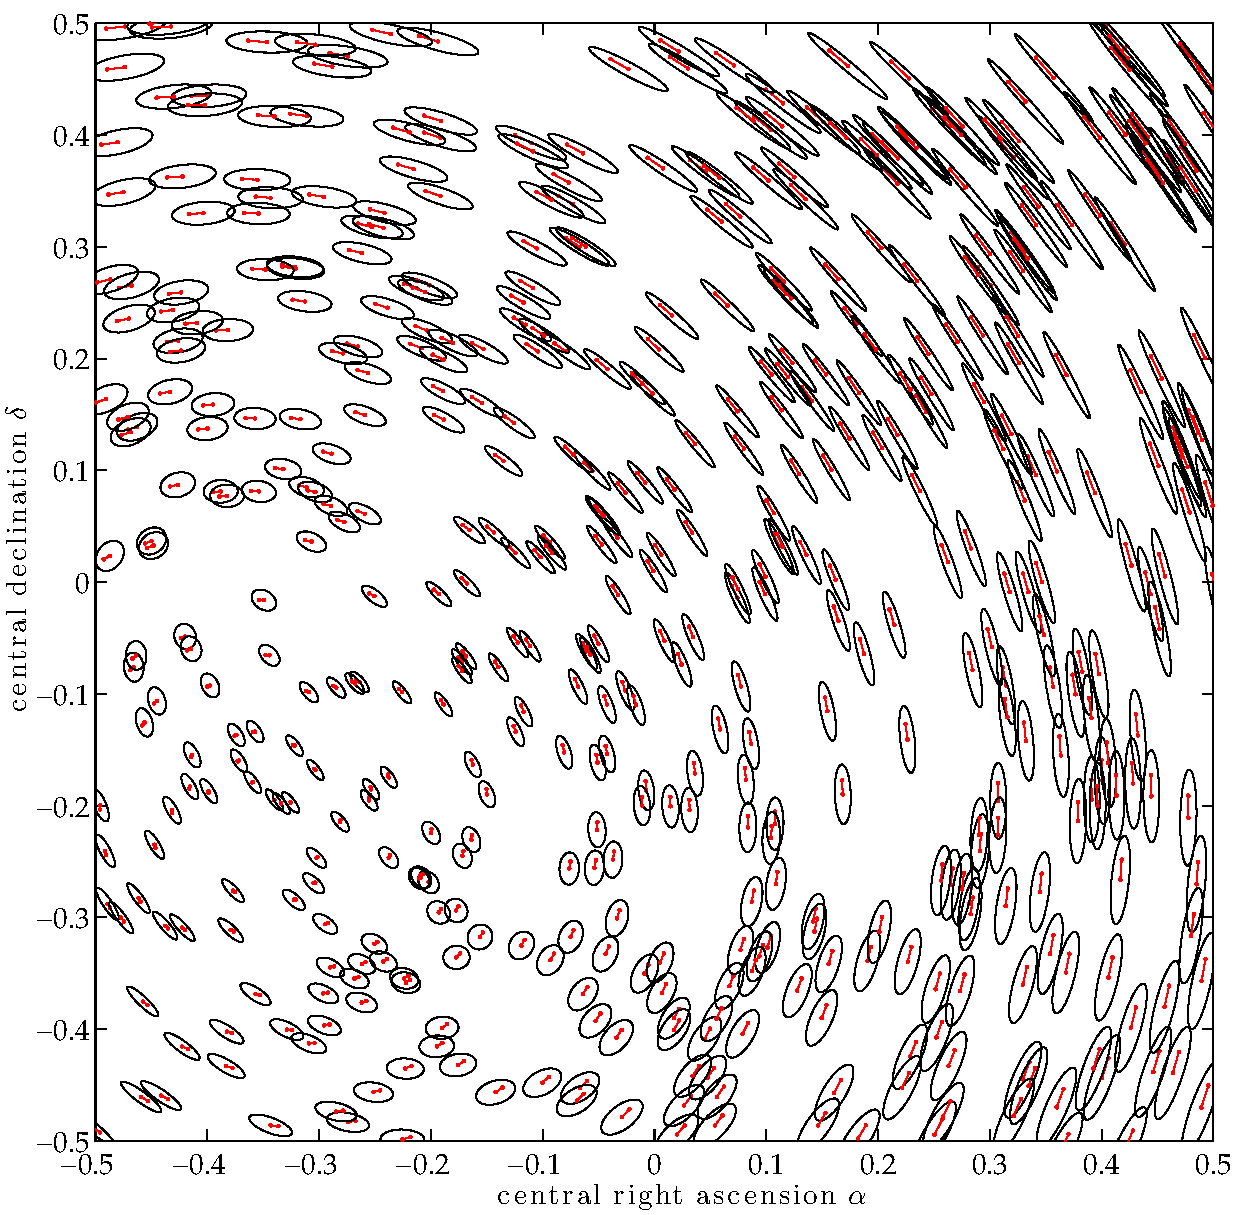
\includegraphics[width=\linewidth]{figures/distortion_map.pdf}
\caption{Distortion map corresponding to the likelihood distribution computer for the mock data. A random distribution of 500 points within the plane (off-centred red points) are mapped to a set of distributions (ellipses) with widths determined by the uncertainty in the mapping space.}\label{fig:map}
\end{figure}
With the chain that has been generated, any point within the image plane can be mapped to a set of transformed points, one for each step in the chain. The spread of these mapped points within the image plane can be used to define the distortion distribution, here assumed to be bivariate normal. Figure~\ref{fig:map} shows this transformation for many such points within the plane.
\footnote{The MCMC run should be `thinned' using only every $n$th member of the chain for some $n>1$. The motivation for this is the adjacent steps in the chain may be correlated and so the inclusion of all steps is non representative of the variance across the entire run. With this distortion map, the scale of the ellipses does increase as the chain is thinned. The map shown here is with quite substantial thinning; if no thinning is used the scale of the distortion distribution for each point is much smaller. I'm not sure whether this is to be regarded as correct (in that correlation in the chain is being removed) or wrong (in that the distortion map should be insensitive to thinning). }

\subsection{High proper motion white dwarf}

\subsection{Adam's data}

\section{Discussion}

\subsection{Likelihood folding for proper motion and parallax}

\subsection{Bayesian cross-validation and false matches}

\section{Conclusion}
We have produced a scheme for determining the likelihood distribution of mappings composed of translations, scalings and rotations between two frames in which tie objects are characterised by known bivariate normal distributions. MCMC is used to explore the likelihood distribution, which is found to be well described by a multivariate gaussian in the mapping parameters. With this model for the likelihood, a map of the distortion distribution within the image plane has been produced.

\acknowledgments

We acknowledge helpful contributions to this work from: Suzanne Aigrain, Henrik Brink, David Hogg, Ryan O'Leary, Matt McQuinn, John Rice, Joey Richards \& Dan Starr. 

\bibliographystyle{apj}
\bibliography{BA}
%\begin{thebibliography}{}
%\bibitem[Barron et al.(2008)]{2008AJ....136.1490B} Barron, J.~T., Hogg, D.~W., Lang, D., \& Roweis, S.\ 2008, \aj, 136, 1490 
%\bibitem[Bertin(2006)]{2006ASPC..351..112B} Bertin, E.\ 2006, Astronomical 
%Data Analysis Software and Systems XV, 351, 112 
%\bibitem[Bertin et al.(2002)]{2002ASPC..281..228B} Bertin, E., Mellier, Y., 
%Radovich, M., et al.\ 2002, Astronomical Data Analysis Software and Systems 
%XI, 281, 228 
%\bibitem[Bonilla, Chai \& Williams(2008)]{bonilla08} Bonilla, E.~V., Chai, K.~M.~A., \& Williams, C.~K.~I. (2008), in Advances in Neural Information Processing Systems 20, Eds. J.~C.~Platt, D.~Koller, Y.~Singer, S.~Roweis, MIT Press
%\bibitem[Boyle \& Frean (2005)]{BF2005} Boyle, P., \& Frean, M. 2005, Advances in Neural Information Processing Systems 17 217-224
%\bibitem[Calabretta \& Greisen(2002)]{2002A&A...395.1077C} Calabretta, M.~R., \& Greisen, E.~W.\ 2002, \aap, 395, 1077 
%\bibitem[Cressie (1993)]{Cressie1993} Cressie, N.A.C. 1993, Statistics for spatial data, J. Wiley
%\bibitem[Greisen \& Calabretta(2002)]{2002A&A...395.1061G} Greisen, E.~W., \& Calabretta, M.~R.\ 2002, \aap, 395, 1061 
%\bibitem[Greisen et al.(2006)]{2006A&A...446..747G} Greisen, E.~W., Calabretta, M.~R., Valdes, F.~G., \& Allen, S.~L.\ 2006, \aap, 446, 747 
%\bibitem[Groth(1986)]{1986AJ.....91.1244G} Groth, E.~J.\ 1986, \aj, 91, 
%1244 
%\bibitem[Lang et al.(2009)]{2009AJ....137.4400L} Lang, D., Hogg, D.~W., Jester, S., \& Rix, H.-W.\ 2009, \aj, 137, 4400 
%\bibitem[Lang et al.(2010)]{2010AJ....139.1782L} Lang, D., Hogg, D.~W., Mierle, K., Blanton, M., \& Roweis, S.\ 2010, \aj, 139, 1782 
%\bibitem[Makarov et al.(2012)]{2012PASP..124..268M} Makarov, V.~V., Veillette, D.~R., Hennessy, G.~S., \& Lane, B.~F.\ 2012, \pasp, 124, 268
%\bibitem[{Rasmussen and Williams(2006)}]{raswil06} Rasmussen, C., Williams, C., 2006. Gaussian processes for machine learning. MIT Press.
%\bibitem[Zacharias et al.(2004)]{2004AJ....127.3043Z} Zacharias, N., Urban, S.~E., Zacharias, M.~I., et al.\ 2004, \aj, 127, 3043 
%\end{thebibliography}

\appendix

\section{Tutorial: probabilistic astrometry software}
\subsection{Interactive mode}
\subsection{Command line mode}

\section{Implementation details}

\end{document}

